\chapter{रासायनिक विभव और मिश्रण}\label{ch:b2:chemical-potential}

सर्दियों में एक ट्रक बर्फ़ीली सड़क पर नमक बिखेरता है और बर्फ़
\qty{-10}{\celsius} पर पिघल जाती है; कार इंजन का शीतलक, जिसमें पानी के साथ एक-तिहाई
एथेन-1,2-डाइऑल होता है, न रात के पाले में जमता है, न गर्म बोनट के नीचे
उबलता है। घुला हुआ पदार्थ अपने विलायक का हिमांक घटाता है और
क्वथनांक बढ़ाता है, और तनु विलयनों के लिए यह परिवर्तन घुले हुए कणों की
संख्या पर निर्भर करता है, उनकी प्रकृति पर नहीं। इसकी व्याख्या करने वाला
साधन \omterm{def:b2:chemical-potential:chemical-potential}{रासायनिक विभव} है, जो किसी एक घटक की मात्रा के सापेक्ष \omterm{def:b2:reaction-free-energy:gibbs-energy}{गिब्स ऊर्जा}
का आंशिक अवकलज है। यह बताता है कि हर स्पीशीज़ प्रावस्थाओं के बीच और
अभिक्रियाओं के द्वारा ``कहाँ जाना चाहती है'', और उन सक्रियताओं को, जिन्हें
प्रथम वर्ष के खंड ने नुस्खों की तरह प्रयुक्त किया था, व्युत्पन्न राशियाँ बना देता है।

\begin{recall}
\Cref{ch:b2:reaction-free-energy}: \omterm{def:b2:reaction-free-energy:gibbs-energy}{गिब्स ऊर्जा} $G = H - TS$, $\dd G =
V\dd p - S\dd T + \Delta_r G\,\dd\xi$, विकास निकष $\Delta_r G\,
\dd\xi \leq 0$। प्रथम वर्ष के खंड ने गैस की सक्रियता
$p_i/p^\circ$, विलेय की $c_i/c^\circ$, और शुद्ध ठोस या
विलायक की 1 लिखी थी, और कहा था कि सांद्र आयनिक विलयनों में सक्रियताएँ
सांद्रताओं से हट जाती हैं, ``एक संशोधन जिसे द्वितीय वर्ष के खंड में देखा जाएगा''।
भौतिकी से: आदर्श-गैस नियम, और शुद्ध पदार्थ के लिए
$(\partial G/\partial p)_T = V$।
\end{recall}

\begin{omfigure}
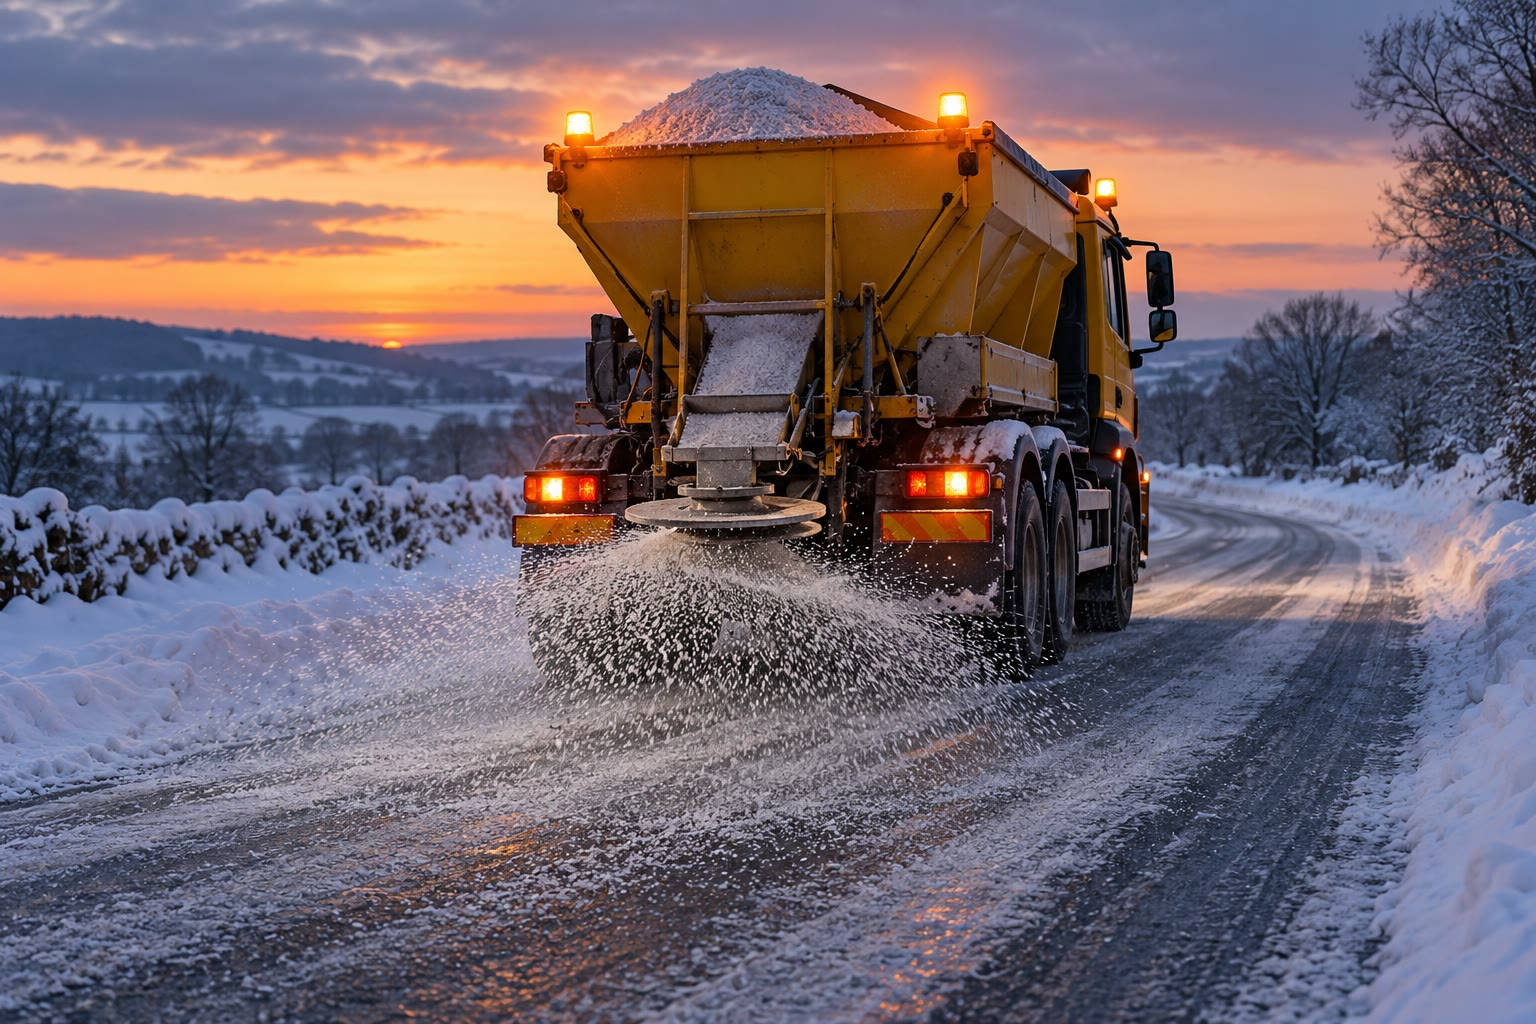
\includegraphics[width=0.58\linewidth]{images/book3/ai/b2-03-salt-spreader.jpg}

{\small एक ट्रक बर्फ़ से ढकी सड़क पर नमक बिखेरता है। नमक बर्फ़ पर पानी की
पतली परत में घुलता है, और विलयन शुद्ध पानी से कम ताप पर
जमता है: बर्फ़ पिघल जाती है।}
\end{omfigure}

\section{आंशिक मोलर राशियाँ}

\qty{50}{mL} पानी और \qty{50}{mL} एथेनॉल मिलाइए: मिश्रण का आयतन
\qty{100}{mL} से कम होता है। किसी मिश्रण में कोई विस्तीर्ण राशि
शुद्ध पदार्थों के योगदानों का योग नहीं होती; हर घटक
अपने परिवेश के अनुसार योगदान करता है।

\begin{definition}[आंशिक मोलर राशि]\label{def:b2:chemical-potential:partial-molar}
मान लीजिए $X(T, p, n_1, \dots, n_k)$ ऐसी प्रावस्था का एक विस्तीर्ण अवस्था फलन है
जिसमें मात्राएँ $n_1, \dots, n_k$ हैं। घटक $i$ की \emph{आंशिक मोलर
राशि}\index{आंशिक मोलर राशि} यह है:
\[
  \bar X_i = \left(\frac{\partial X}{\partial n_i}\right)_{T, p, n_{j \ne i}} ,
\]
अर्थात् $X$ का वह परिवर्तन जो मिश्रण की बड़ी मात्रा में $i$ का एक मोल मिलाने पर होता है,
नियत $T$, $p$ और अन्य मात्राओं पर। $X = V$ के लिए यह \emph{आंशिक
मोलर आयतन}\index{आंशिक मोलर आयतन} $\bar V_i$ है।
\end{definition}

\begin{theorem}[ऑयलर सर्वसमिका]\label{thm:b2:chemical-potential:euler}
नियत $T$ और $p$ पर $X = \sum_i n_i\bar X_i$।
\end{theorem}

\begin{proof}\emergencystretch=3em
$X$ विस्तीर्ण है: हर मात्रा को $\lambda$ से गुणा करने पर $X$ भी
$\lambda$ से गुणा होता है, $X(T, p, \lambda n_1, \dots, \lambda n_k) = \lambda X(T, p, n_1,
\dots, n_k)$। $\lambda$ के सापेक्ष, $\lambda = 1$ पर, अवकलन कीजिए,
शृंखला नियम से: $\sum_i n_i\,\partial X/\partial n_i = X$।
\end{proof}

\begin{proposition}[गिब्स--ड्यूहेम संबंध]\label{prop:b2:chemical-potential:gibbs-duhem}
नियत $T$ और $p$ पर $\sum_i n_i\,\dd\bar X_i = 0$: द्वि-घटकी मिश्रण में
$x_1\dd\bar X_1 + x_2\dd\bar X_2 = 0$। घटकों की \omterm{def:b2:chemical-potential:partial-molar}{आंशिक मोलर राशियाँ}
स्वतंत्र रूप से नहीं बदल सकतीं।
\end{proposition}

\begin{proof}
नियत $T$, $p$ पर परिभाषा से $\dd X = \sum_i\bar X_i\dd n_i$; ऑयलर
सर्वसमिका का अवकलन $\dd X = \sum_i\bar X_i\dd n_i + \sum_i
n_i\dd\bar X_i$ देता है। घटाइए।
\end{proof}

\begin{omfigure}
\begin{tikzpicture}
\begin{axis}[
  width=0.62\linewidth, height=5.4cm, xmin=0, xmax=1, ymin=8, ymax=62,
  axis x line=bottom, axis y line=left, xlabel={मोल अंश $x_2$},
  ylabel={मोलर आयतन $V_m$ (मॉडल)}, xtick={0,0.2,0.4,0.6,0.8,1}, ytick=\empty, ylabel shift=10pt,
  tick label style={font=\small}, label style={font=\small}, clip=false]
\addplot[omDef, very thick, domain=0:1, samples=60] {18*(1-x) + 58*x - 25*x*(1-x)};
\addplot[black!40, dashed, domain=0:1] {18*(1-x) + 58*x};
\addplot[omThm, thick, domain=0:1] {14 + 35*x};
\fill[omThm] (axis cs:0.4,28) circle (1.6pt);
\node[omThm, anchor=east, font=\small] at (axis cs:-0.01,14) {$\bar V_1$};
\node[omThm, anchor=west, font=\small] at (axis cs:1,49) {$\bar V_2$};
\node[font=\scriptsize, anchor=south east, black!60] at (axis cs:0.62,44) {शुद्ध आयतनों का योग};
\node[font=\small, anchor=north west] at (axis cs:0.41,27) {$x_2 = 0.4$};
\end{axis}
\end{tikzpicture}

{\small स्पर्शरेखा रचना। किसी मॉडल द्वि-घटकी मिश्रण का मोलर आयतन
(नीला) शुद्ध आयतनों को जोड़ने वाली सरल रेखा से नीचे है: मिश्रण
संकुचित होता है। किसी संघटन पर स्पर्शरेखा दोनों किनारों को उस संघटन के \omterm{def:b2:chemical-potential:partial-molar}{आंशिक
मोलर आयतनों} $\bar V_1$ और $\bar V_2$ पर काटती है।}
\end{omfigure}

\begin{method}[वक्र से आंशिक मोलर राशियाँ]\label{met:b2:chemical-potential:tangent}
मोलर राशि $X_m = X/(n_1 + n_2)$ को $x_2$ के सापेक्ष आलेखित कीजिए। वांछित
संघटन पर स्पर्शरेखा खींचिए: यह अक्ष $x_2 = 0$ को
$\bar X_1$ पर और अक्ष $x_2 = 1$ को $\bar X_2$ पर काटती है। (उपपत्ति: $X_m = x_1\bar X_1 +
x_2\bar X_2$ और, गिब्स--ड्यूहेम से, $\dd X_m/\dd x_2 = \bar X_2 - \bar X_1$।)
\end{method}

\section{रासायनिक विभव}

\begin{definition}[रासायनिक विभव]\label{def:b2:chemical-potential:chemical-potential}
किसी प्रावस्था में घटक $i$ का \emph{रासायनिक विभव}\index{रासायनिक विभव}
उसकी आंशिक मोलर \omterm{def:b2:reaction-free-energy:gibbs-energy}{गिब्स ऊर्जा} है,
\[
  \mu_i = \left(\frac{\partial G}{\partial n_i}\right)_{T, p, n_{j\ne i}} ,
\]
\unit{J/mol} में। जब $i$ अपनी मानक अवस्था में हो, तब इसका मान उसका
\emph{मानक रासायनिक विभव}\index{मानक रासायनिक विभव}
$\mu_i^\circ(T)$ है, जो $i$ की मानक मोलर \omterm{def:b2:reaction-free-energy:gibbs-energy}{गिब्स ऊर्जा} के बराबर है।
\end{definition}

ऐसी प्रावस्था के लिए जिसकी मात्राएँ बदल सकती हैं (अभिक्रिया से, या किसी
दूसरी प्रावस्था के साथ विनिमय से),
\[
  \dd G = V\dd p - S\dd T + \sum_i\mu_i\,\dd n_i ,\qquad G = \sum_i n_i\mu_i ,
\]
दूसरा संबंध ऑयलर सर्वसमिका से। एक ही अभिक्रिया होने पर $\dd n_i =
\nu_i\dd\xi$, और \cref{prop:b2:reaction-free-energy:dG} से तुलना करने पर:
\[
  \Delta_r G = \sum_i\nu_i\mu_i .
\]
\omterm{def:b2:reaction-free-energy:reaction-gibbs}{अभिक्रिया गिब्स ऊर्जा} उत्पादों और अभिकारकों के \omterm{def:b2:chemical-potential:chemical-potential}{रासायनिक विभवों} का
संतुलन है।

\begin{theorem}[प्रावस्थाओं के बीच साम्य]\label{thm:b2:chemical-potential:phase-equilibrium}
किसी बंद निकाय की दो प्रावस्थाओं $\alpha$ और $\beta$ में, जिसके $T$ और $p$
एकसमान हैं, उपस्थित कोई घटक उनके बीच साम्य में है यदि और केवल यदि
$\mu_i^\alpha = \mu_i^\beta$। अन्यथा वह उस प्रावस्था से, जहाँ उसका \omterm{def:b2:chemical-potential:chemical-potential}{रासायनिक
विभव} अधिक है, उस प्रावस्था में स्वतः चला जाता है जहाँ वह कम है।
\end{theorem}

\begin{proof}
स्थानांतरण $i^\alpha \to i^\beta$ एक ``अभिक्रिया'' है, जिसमें $\nu^\alpha = -1$,
$\nu^\beta = +1$, अतः $\Delta_r G = \mu_i^\beta - \mu_i^\alpha$। विकास
निकष से यह आगे बढ़ता है ($\dd\xi > 0$) केवल यदि $\mu_i^\beta <
\mu_i^\alpha$, पीछे लौटता है यदि $\mu_i^\beta > \mu_i^\alpha$, और
साम्य में है यदि दोनों बराबर हों।
\end{proof}

द्रव्य के लिए \omterm{def:b2:chemical-potential:chemical-potential}{रासायनिक विभव} वही भूमिका निभाता है जो ऊष्मा के लिए ताप:
ऊष्मा गर्म से ठंडे की ओर बहती है, स्पीशीज़ उच्च से निम्न $\mu$ की ओर।

\section{आदर्श निकाय और सक्रियताएँ}

\begin{proposition}[आदर्श गैस का रासायनिक विभव]\label{prop:b2:chemical-potential:mu-gas}
आदर्श गैसों के मिश्रण में आंशिक दाब $p_i$ वाली गैस के लिए
\[
  \mu_i = \mu_i^\circ(T) + RT\ln\frac{p_i}{p^\circ} .
\]
\end{proposition}

\begin{proof}
शुद्ध आदर्श गैस के एक मोल के लिए $(\partial\mu/\partial p)_T = V_m =
RT/p$; $p^\circ$ से $p$ तक समाकलन करने पर $\mu = \mu^\circ + RT\ln(p/p^\circ)$ मिलता है।
आदर्श गैसों के मिश्रण में हर गैस आयतन में अकेली होने जैसा, अपने
आंशिक दाब पर, व्यवहार करती है: $p$ की जगह $p_i$ रखिए।
\end{proof}

\begin{definition}[आदर्श मिश्रण, आदर्श तनु विलयन]\label{def:b2:chemical-potential:ideal-mixture}
कोई द्रव (या ठोस) मिश्रण \emph{आदर्श मिश्रण}\index{आदर्श मिश्रण} है
यदि हर घटक और हर संघटन के लिए
$\mu_i = \mu_i^*(T, p) + RT\ln x_i$, जहाँ $\mu_i^*$ शुद्ध द्रव $i$ का \omterm{def:b2:chemical-potential:chemical-potential}{रासायनिक
विभव} है। कोई विलयन \emph{आदर्श तनु
विलयन}\index{आदर्श तनु विलयन} है यदि विलायक इस नियम का पालन करे और हर
विलेय $\mu_j = \mu_j^\circ(T) + RT\ln(c_j/c^\circ)$ का पालन करे, जहाँ मानक
अवस्था $c^\circ = \qty{1}{mol/L}$ पर एक काल्पनिक विलयन है जो अनंत तनु
होने जैसा व्यवहार करता है।
\end{definition}

समान आकार और आकृति वाले ऐसे अणु, जिनकी अन्योन्यक्रियाएँ साथी पर निर्भर नहीं करतीं
(बेन्ज़ीन और टॉलूईन, किसी अणु के दो समस्थानिकी रूप), लगभग
\omterm{def:b2:chemical-potential:ideal-mixture}{आदर्श मिश्रण} बनाते हैं; तनु विलयन आदर्श व्यवहार करते हैं क्योंकि हर विलेय
कण केवल विलायक से घिरा होता है।

\begin{theorem}[राउल्ट का नियम]\label{thm:b2:chemical-potential:raoult}
किसी आदर्श द्रव मिश्रण के ऊपर, वाष्प को आदर्श गैस मानने पर, हर घटक का आंशिक
दाब द्रव में उसके मोल अंश के समानुपाती होता है:
$p_i = x_i\,p_i^*$, जहाँ $p_i^*$ उसी ताप पर शुद्ध द्रव का वाष्प दाब
है (\emph{राउल्ट का नियम}\index{राउल्ट का नियम})।
\end{theorem}

\begin{proof}
साम्य पर $\mu_i(\text{द्रव}) = \mu_i(\text{वाष्प})$: $\mu_i^* +
RT\ln x_i = \mu_i^\circ + RT\ln(p_i/p^\circ)$। शुद्ध द्रव के लिए ($x_i = 1$,
$p_i = p_i^*$): $\mu_i^* = \mu_i^\circ + RT\ln(p_i^*/p^\circ)$। घटाने पर
$RT\ln x_i = RT\ln(p_i/p_i^*)$। (दाब पर $\mu_i^*$ की दुर्बल निर्भरता
नगण्य मानी गई है।)
\end{proof}

\begin{proposition}[हेनरी का नियम]\label{prop:b2:chemical-potential:henry}
अपनी वाष्प के साथ साम्य में किसी तनु विलेय $j$ के लिए $p_j = k_{H,j}\,x_j$
(या $c_j = H_j\,p_j$): तनु विलेय का आंशिक दाब विलयन में उसकी मात्रा के
समानुपाती होता है (\emph{हेनरी का
नियम}\index{हेनरी का नियम})। \emph{हेनरी स्थिरांक}\index{हेनरी स्थिरांक}
$k_{H,j}$ विलेय, विलायक और ताप पर निर्भर करता है, और वह
शुद्ध विलेय का वाष्प दाब नहीं है।
\end{proposition}

\begin{proof}
$\mu_j^\circ(\text{विलयन}) + RT\ln(c_j/c^\circ)$ और
$\mu_j^\circ(\text{गैस}) + RT\ln(p_j/p^\circ)$ को बराबर रखिए: $c_j/p_j$ केवल
$T$ का फलन है। स्थिरांक में $j$ की विलायक के साथ अन्योन्यक्रियाएँ हैं,
स्वयं अपने साथ नहीं।
\end{proof}

\begin{omfigure}
\begin{tikzpicture}
\begin{axis}[name=a,
  width=0.48\linewidth, height=5.6cm, xmin=0, xmax=1, ymin=0, ymax=1.5,
  axis x line=bottom, axis y line=left, xlabel={$x_1$}, ylabel={$p/p_1^*$},
  xtick={0,0.5,1}, ytick={0,0.5,1,1.5},
  tick label style={font=\small}, label style={font=\small}, title={\small आदर्श}]
\addplot[omDef, thick] table[x=x1, y=p1] {figdata/out/bachelor-2-raoult-henry-ideal.dat};
\addplot[omThm, thick] table[x=x1, y=p2] {figdata/out/bachelor-2-raoult-henry-ideal.dat};
\addplot[black, very thick] table[x=x1, y=p] {figdata/out/bachelor-2-raoult-henry-ideal.dat};
\node[omDef, font=\scriptsize, anchor=west] at (axis cs:0.55,0.42) {$p_1$};
\node[omThm, font=\scriptsize, anchor=west] at (axis cs:0.1,0.42) {$p_2$};
\node[font=\scriptsize, anchor=south] at (axis cs:0.5,0.8) {$p$};
\end{axis}
\begin{axis}[at={(a.east)}, anchor=west, xshift=1.2cm,
  width=0.48\linewidth, height=5.6cm, xmin=0, xmax=1, ymin=0, ymax=1.5,
  axis x line=bottom, axis y line=left, xlabel={$x_1$},
  xtick={0,0.5,1}, ytick={0,0.5,1,1.5},
  tick label style={font=\small}, label style={font=\small}, title={\small धनात्मक विचलन}]
\addplot[omDef, thick] table[x=x1, y=p1] {figdata/out/bachelor-2-raoult-henry-margules.dat};
\addplot[omThm, thick] table[x=x1, y=p2] {figdata/out/bachelor-2-raoult-henry-margules.dat};
\addplot[black, very thick] table[x=x1, y=p] {figdata/out/bachelor-2-raoult-henry-margules.dat};
\addplot[omDef, densely dashed, domain=0.6:1] {x};
\addplot[omDef, dotted, thick, domain=0:0.42] {3.004166*x};
\node[omDef, font=\scriptsize, anchor=west] at (axis cs:0.62,0.5) {राउल्ट};
\node[omDef, font=\scriptsize, anchor=east] at (axis cs:0.27,1.18) {हेनरी};
\node[omDef, font=\scriptsize, anchor=north west] at (axis cs:0.8,0.78) {$p_1$};
\node[omThm, font=\scriptsize, anchor=north] at (axis cs:0.55,0.24) {$p_2$};
\node[font=\scriptsize, anchor=south] at (axis cs:0.5,1.23) {$p$};
\end{axis}
\end{tikzpicture}

{\small नियत ताप पर किसी द्वि-घटकी द्रव के ऊपर वाष्प दाब, $p_1^*$ की
इकाइयों में (मॉडल मिश्रण)। बाएँ, \omterm{def:b2:chemical-potential:ideal-mixture}{आदर्श मिश्रण}: सरल रेखाएँ (राउल्ट)।
दाएँ, ऐसा मिश्रण जिसके असमान अणु एक-दूसरे को समान अणुओं से कम आकर्षित
करते हैं: दाब आदर्श रेखाओं से ऊपर हैं। $x_1 = 1$ के निकट घटक 1
राउल्ट की रेखा (खंडित) का अनुसरण करता है; $x_1 = 0$ के निकट वह भिन्न
प्रवणता वाली हेनरी रेखा (बिंदुकित) का।}
% (computed in figdata/bachelor-2/raoult-henry.py; Margules parameter 1.1, model)
\end{omfigure}

\begin{example}[सोडा में कार्बन डाइऑक्साइड]\label{ex:b2:chemical-potential:soda}
\qty{25}{\celsius} पर पानी में कार्बन डाइऑक्साइड का \omterm{prop:b2:chemical-potential:henry}{हेनरी स्थिरांक} $H =
\qty{3.4e-4}{mol/(m^3.Pa)}$ है, अर्थात् \qty{0.034}{mol/(L.bar)}। \ce{CO2} के
\qty{4}{bar} पर सीलबंद बोतल में $0.034 \times 4 =
\qty{0.14}{mol/L}$ घुली गैस होती है, लगभग \qty{6}{g/L}। खोलने पर उसके
ऊपर की गैस वायु होती है, जहाँ $p_{\ce{CO2}} \approx \qty{4e-4}{bar}$: पेय
दस हज़ार गुना अतिसंतृप्त होता है और तब तक बुदबुदाता है जब तक फीका न पड़ जाए।
% ledger: henry:CO2, air:CO2
\end{example}

\begin{proposition}[रासायनिक विभवों से सक्रियताएँ]\label{prop:b2:chemical-potential:activity}
अब तक की हर स्थिति में $\mu_i = \mu_i^\circ(T) + RT\ln a_i$, जहाँ $a_i$
प्रथम वर्ष के खंड की सक्रियता है: आदर्श गैस के लिए $p_i/p^\circ$,
\omterm{def:b2:chemical-potential:ideal-mixture}{आदर्श तनु विलयन} के विलेय के लिए $c_i/c^\circ$, विलायक के लिए $x_i$ (1 के निकट),
और अपनी प्रावस्था में अकेले शुद्ध ठोस या द्रव के लिए 1।
\end{proposition}

\begin{proof}
गैस और तनु विलेय के लिए यही
\cref{prop:b2:chemical-potential:mu-gas} की और \omterm{def:b2:chemical-potential:ideal-mixture}{आदर्श
तनु विलयन} की परिभाषा की विषयवस्तु है। \omterm{def:b2:chemical-potential:ideal-mixture}{आदर्श मिश्रण} के किसी घटक के लिए उसकी मानक
अवस्था शुद्ध द्रव लीजिए: $a_i = x_i$, जो विलायक के लिए 1 के निकट है। शुद्ध ठोस
या द्रव स्वयं अपनी मानक अवस्था है (दाब पर उसकी दुर्बल निर्भरता
नगण्य मानकर): $\mu = \mu^\circ$, $a = 1$।
\end{proof}

\begin{proposition}[अभिक्रिया गिब्स ऊर्जा और भागफल]\label{prop:b2:chemical-potential:delta-g-q}
किसी अभिक्रिया $0 = \sum_i\nu_i\mathrm A_i$ के लिए,
\[
  \Delta_r G = \Delta_r G^\circ(T) + RT\ln Q, \qquad Q = \prod_i a_i^{\nu_i} .
\]
\end{proposition}

\begin{proof}
$\Delta_r G = \sum_i\nu_i\mu_i = \sum_i\nu_i\mu_i^\circ + RT\sum_i\nu_i\ln a_i =
\Delta_r G^\circ + RT\ln\prod_i a_i^{\nu_i}$.
\end{proof}

यह \cref{ch:b2:reaction-free-energy} की \omterm{def:b2:reaction-free-energy:gibbs-energy}{गिब्स ऊर्जा} और प्रथम वर्ष के खंड
के अभिक्रिया भागफल के बीच का सेतु है। अगला अध्याय इसे पार करता है।

\begin{method}[सक्रियता की संदर्भ अवस्था का चुनाव]\label{met:b2:chemical-potential:activity-reference}
\begin{enumerate}
  \item गैस: $p^\circ$ पर शुद्ध आदर्श गैस; $a = p_i/p^\circ$।
  \item विलायक, या तुलनीय मात्राओं वाले मिश्रण का कोई घटक:
        शुद्ध द्रव; $a = \gamma_i x_i$ (राउल्ट संदर्भ, $\gamma_i \to 1$
        जब $x_i \to 1$)।
  \item विलेय: $c^\circ$ पर आदर्श विलयन; $a = \gamma_j c_j/c^\circ$
        (हेनरी संदर्भ, अनंत तनुता पर $\gamma_j \to 1$)।
  \item शुद्ध ठोस, अपनी प्रावस्था में अकेला शुद्ध द्रव: $a = 1$।
\end{enumerate}
\end{method}

\begin{history}[फ़्रांस्वा-मारी राउल्ट]
\begin{minipage}[t]{0.2\linewidth}\vspace{0pt}
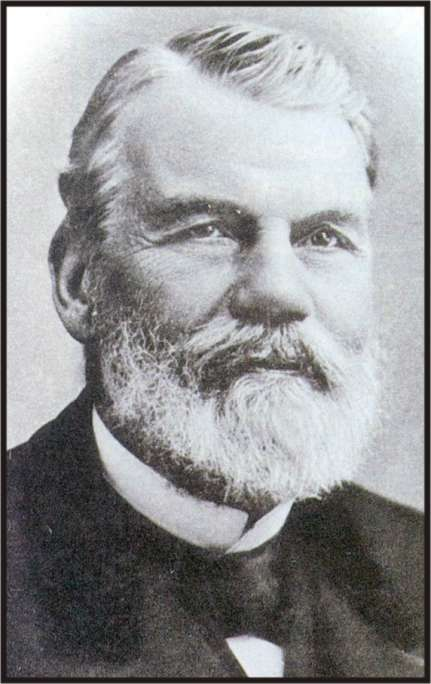
\includegraphics[width=\linewidth]{images/book3/raoult.jpg}
\end{minipage}\hfill
\begin{minipage}[t]{0.76\linewidth}\vspace{0pt}
फ़्रांस्वा-मारी राउल्ट (1830--1901), ग्रेनोबल में रसायन के प्राध्यापक, ने
1880 के दशक में सैकड़ों विलयनों के हिमांक और फिर वाष्प दाब मापे,
और पाया कि तनु विलयनों के लिए यह अवनमन
घुले अणुओं की संख्या पर निर्भर करता है, उनकी प्रकृति पर नहीं। उनके
माप अणुओं को तौलने का एक तरीका बन गए, और उन्होंने विलयन में आयनों के
नए सिद्धांत का समर्थन किया। (छायाचित्र: सार्वजनिक अधिकार-क्षेत्र, विकिमीडिया कॉमन्स।)
\end{minipage}
\end{history}

\section{वास्तविक मिश्रण}

\begin{definition}[सक्रियता गुणांक]\label{def:b2:chemical-potential:activity-coefficient}
वास्तविक मिश्रण में \omterm{def:b2:chemical-potential:chemical-potential}{रासायनिक विभव} $\mu_i = \mu_i^\circ +
RT\ln a_i$ लिखा जाता है, जहाँ $a_i = \gamma_i x_i$ (राउल्ट संदर्भ) या $a_i = \gamma_i
c_i/c^\circ$ (हेनरी संदर्भ)। गुणक $\gamma_i$ \emph{सक्रियता
गुणांक}\index{सक्रियता गुणांक} है: यह आदर्श नियम से विचलन मापता है, और
उस सीमा में 1 की ओर प्रवृत्त होता है जहाँ संदर्भ नियम लागू होता है।
\end{definition}

1 से बड़े गुणांक का अर्थ है कि अणु मिश्रण में अपने पड़ोसियों द्वारा संदर्भ
अवस्था की तुलना में कम स्थायीकृत होता है (धनात्मक विचलन, जैसा ऊपर के चित्र
में); 1 से छोटे का अर्थ है अधिक स्थायीकृत। गिब्स--ड्यूहेम से द्वि-घटकी मिश्रण के
दोनों घटकों के गुणांक जुड़े होते हैं: चित्र के लिए प्रयुक्त एक-प्राचल
मॉडल में $\ln\gamma_1 = Ax_2^2$ और $\ln\gamma_2 = Ax_1^2$, और
$x_1\,\dd\ln\gamma_1 + x_2\,\dd\ln\gamma_2 = 0$ सर्वसमिका के रूप में सत्य है।

आयनों के लिए, जो लंबी दूरी तक अन्योन्यक्रिया करते हैं, विचलन छोटी
सांद्रताओं पर ही प्रकट हो जाते हैं।

\begin{definition}[आयनिक सामर्थ्य]\label{def:b2:chemical-potential:ionic-strength}
किसी विलयन की \emph{आयनिक सामर्थ्य}\index{आयनिक सामर्थ्य} $I =
\frac12\sum_i z_i^2\,b_i$ है, जहाँ $b_i$ आयन $i$ की मोललता (प्रति
किलोग्राम विलायक मात्रा) है और $z_i$ उसकी आवेश संख्या।
\end{definition}

\begin{proposition}[डिबाई--ह्युकेल सीमांत नियम]\label{prop:b2:chemical-potential:debye-huckel}
अति तनु विद्युत-अपघट्य विलयन में किसी लवण के आयनों का माध्य
\omterm{def:b2:chemical-potential:activity-coefficient}{सक्रियता गुणांक} $\log\gamma_\pm = -A\,|z_+z_-|\sqrt{I/b^\circ}$ का पालन करता है, जहाँ
\qty{25}{\celsius} पर जल के लिए $A
\approx 0.51$ और $b^\circ =
\qty{1}{mol/kg}$।
\end{proposition}
\admitted

\begin{remark}[परिसर और उद्गम]\label{rem:b2:chemical-potential:dh-range}
यह नियम एक मॉडल से आता है जिसमें हर आयन विपरीत आवेश के एक विसरित
``वायुमंडल'' से घिरा होता है, जो उसका \omterm{def:b2:chemical-potential:chemical-potential}{रासायनिक विभव} घटा देता है;
मॉडल इस पाठ्यक्रम से परे है, परंतु उसका स्थिरांक $A$ जल की
विद्युतशीलता और घनत्व तथा ताप से निकलता है। यह लगभग
$I = \qty{0.01}{mol/kg}$ से नीचे यथार्थ है। यही आयनिक वायुमंडल विद्युत क्षेत्र में
आयनों को धीमा करता है, और समझाता है कि प्रबल विद्युत-अपघट्य की मोलर चालकता
अपने सीमांत मान पर टिके रहने के बजाय $\Lambda = \Lambda^\circ - K\sqrt c$
(कोलराउश का वर्गमूल नियम) के अनुसार क्यों घटती है: यही प्रथम वर्ष के
खंड में मिले कोलराउश नियम की सीमा है।
% ledger: epsr:H2O, rho:water.298, const:e, const:eps0, const:kB, const:NA (A computed in figdata/bachelor-2/colligative.py)
\end{remark}

\begin{example}[एक सेंटीमोलर लवण]\label{ex:b2:chemical-potential:dh}
$b = \qty{0.010}{mol/kg}$ पर सोडियम क्लोराइड के लिए $I = \frac12(0.010 + 0.010)
= \qty{0.010}{mol/kg}$ और $\log\gamma_\pm = -0.51 \times 0.10$: $\gamma_\pm
= 0.89$। मोल प्रति किलोग्राम के सौवें भाग पर ही सक्रियता के स्थान पर
सांद्रता लेना 11\,\% की त्रुटि है; उसी मोललता पर मैग्नीशियम सल्फ़ेट जैसे
2:2 लवण के लिए $I = 0.040$ और $\gamma_\pm = 0.62$।
\end{example}

\section{अणुसंख्य गुणधर्म}

\begin{definition}[अणुसंख्य गुणधर्म]\label{def:b2:chemical-potential:colligative}
किसी तनु विलयन का \emph{अणुसंख्य गुणधर्म}\index{अणुसंख्य गुणधर्म} वह
गुणधर्म है जो विलायक की प्रति मात्रा घुले कणों की मात्रा पर निर्भर करता है,
उनकी प्रकृति पर नहीं: वाष्प दाब का अवनमन, हिमांक का अवनमन,
क्वथनांक का उन्नयन, और \omterm{def:b2:chemical-potential:osmotic-pressure}{परासरण दाब}। नीचे के हिमांक और क्वथनांक
नियमों के स्थिरांक विलायक के \emph{हिमांकमितीय स्थिरांक}\index{हिमांकमितीय स्थिरांक} $K_f$
और \emph{क्वथनांकमितीय स्थिरांक}\index{क्वथनांकमितीय स्थिरांक} $K_b$
हैं।
\end{definition}

\begin{omfigure}
\begin{tikzpicture}[font=\small, >={Stealth}]
  \draw[->] (0,0) -- (8,0) node[right] {$T$};
  \draw[->] (0,0) -- (0,4.4) node[above] {विलायक का $\mu$};
  % slopes = -S_m: the liquid, more disordered, falls faster than the solid
  \draw[omDef, very thick] (0.4,3.0) -- (7.0,2.01) node[right] {ठोस};
  \draw[omThm, very thick] (0.4,3.6) -- (7.6,0.72) node[right] {शुद्ध द्रव};
  \draw[omThm, very thick, dashed] (0.4,3.25) -- (7.6,0.37) node[right] {विलयन};
  \fill (2.8,2.64) circle (1.5pt);
  \fill (1.4,2.85) circle (1.5pt);
  \draw[densely dotted] (2.8,2.64) -- (2.8,0) node[below] {$T_f^*$};
  \draw[densely dotted] (1.4,2.85) -- (1.4,0) node[below] {$T_f$};
  \draw[<->] (1.4,-0.75) -- (2.8,-0.75) node[midway, below] {$\Delta T_f$};
  \draw[<->, black!70] (5.0,1.76) -- (5.0,1.41);
  \draw[black!50] (5.0,1.58) -- (4.6,0.75) node[below, font=\scriptsize, black] {$RT\ln x_1$};
\end{tikzpicture}

{\small ताप के सापेक्ष विलायक का \omterm{def:b2:chemical-potential:chemical-potential}{रासायनिक विभव} (व्यवस्था-चित्र,
नियत दाब पर)। स्थायी प्रावस्था वह है जिसका $\mu$ सबसे कम हो। विलेय घोलने से
द्रव की रेखा $RT\ln x_1 < 0$ से नीचे आ जाती है; अब वह ठोस की रेखा से
कम ताप पर मिलती है: विलयन शुद्ध विलायक से नीचे जमता है।}
\end{omfigure}

\begin{theorem}[हिमांक का अवनमन]\label{thm:b2:chemical-potential:cryoscopy}
ऐसे विलेय का तनु विलयन, जो ठोस में प्रवेश नहीं करता,
$T_f = T_f^* - \Delta T_f$ पर जमना आरंभ करता है, जहाँ
\[
  \Delta T_f = K_f\,b, \qquad K_f = \frac{R\,T_f^{*2}\,M_1}{\Delta_{\text{गलन}}H_1} ,
\]
$b$ घुले कणों की कुल मोललता है और $M_1$ विलायक का मोलर
द्रव्यमान (\unit{kg/mol} में)। परिमित सांद्रताओं के लिए आदर्श विलयन का यथातथ
संबंध $\ln x_1 = -\frac{\Delta_{\text{गलन}}H_1}{R}
\left(\frac{1}{T_f} - \frac{1}{T_f^*}\right)$ है।
\end{theorem}

\begin{proof}\emergencystretch=3em
हिमांक पर शुद्ध ठोस विलायक और विलयन में विलायक
साम्य में होते हैं: $\mu_1^{\text{s}}(T) = \mu_1^{*\text{l}}(T) + RT\ln x_1$, अतः
$\ln x_1 = -\Delta_{\text{गलन}}G_1(T)/(RT)$, जहाँ $\Delta_{\text{गलन}}G_1 =
\mu_1^{*\text{l}} - \mu_1^{\text{s}}$, जो $T_f^*$ पर शून्य है। गिब्स--हेल्महोल्ट्ज़ से
$\dd(\Delta_{\text{गलन}}G_1/T)/\dd T = -\Delta_{\text{गलन}}H_1/T^2$;
$T_f^*$ से $T_f$ तक, $\Delta_{\text{गलन}}H_1$ को स्थिर रखकर, समाकलन करने पर
यथातथ संबंध मिलता है। तनु विलयन के लिए $\ln x_1 = \ln(1 - x_2) \approx
-x_2$ और $\frac1{T_f} - \frac1{T_f^*} \approx -\Delta T_f/T_f^{*2}$, अतः
$x_2 = \Delta_{\text{गलन}}H_1\Delta T_f/(RT_f^{*2})$; अंततः $x_2 \approx
n_2/n_1 = b\,M_1$।
\end{proof}

\begin{proposition}[क्वथनांक का उन्नयन]\label{prop:b2:chemical-potential:ebullioscopy}
अवाष्पशील विलेय का तनु विलयन $T_b^* + \Delta T_b$ पर उबलता है, जहाँ
$\Delta T_b = K_b\,b$, $K_b = RT_b^{*2}M_1/\Delta_{\text{वाष्पन}}H_1$।
\end{proposition}

\begin{proof}
वही, ठोस के स्थान पर वाष्प के साथ: $\mu_1^{*\text{l}} +
RT\ln x_1 = \mu_1^{\text{v}}$; विलायक की रेखा नीचे आती है, और अब वह
वाष्प की रेखा से उच्चतर ताप पर मिलती है।
\end{proof}

\begin{example}[जल]\label{ex:b2:chemical-potential:water-constants}
\qty{273.15}{K} पर $\Delta_{\text{गलन}}H = \qty{333.4}{J/g} = \qty{6.007}{kJ/mol}$
के साथ: $K_f = 8.314 \times 273.15^2 \times 0.018015/6007 =
\qty{1.86}{K.kg/mol}$। \qty{373.12}{K} पर $\Delta_{\text{वाष्पन}}H = \qty{40.65}{kJ/mol}$
के साथ: $K_b = \qty{0.513}{K.kg/mol}$। समुद्री जल, प्रति किलोग्राम \qty{35}{g} लवण,
जिसे सोडियम क्लोराइड गिना जाए (प्रति सूत्र दो कण):
$b = 2 \times 35/58.44/0.965 = \qty{1.24}{mol/kg}$, अतः तनु नियम
\qty{-2.3}{\celsius} का पूर्वानुमान देता है, जो अति-आकलन है: इस सांद्रता पर
आयन आदर्श से बहुत दूर हैं, और समुद्री लवण पूरा सोडियम क्लोराइड नहीं है।
% ledger: dfus:H2O, tfus:H2O, dvap:H2O.nbp, tb:H2O.atm, sea:salinity (computed in figdata/bachelor-2/colligative.py)
\end{example}

\begin{definition}[अर्धपारगम्य झिल्ली, परासरण दाब]\label{def:b2:chemical-potential:osmotic-pressure}
\emph{अर्धपारगम्य झिल्ली}\index{अर्धपारगम्य झिल्ली} विलायक को
गुज़रने देती है, विलेय को नहीं। जब यह किसी विलयन को
शुद्ध विलायक से अलग करती है, तो विलायक विलयन में बहता है; \emph{परासरण
दाब}\index{परासरण दाब} $\Pi$ वह अतिरिक्त दाब है जो उस प्रवाह को रोकने के लिए
विलयन पर लगाना पड़ता है।
\end{definition}

\begin{theorem}[वांट हॉफ़ का परासरण नियम]\label{thm:b2:chemical-potential:osmosis}
तनु विलयन के लिए $\Pi = c\,RT$, जहाँ $c$ विलेय कणों की कुल
सांद्रता है।
\end{theorem}

\begin{proof}
साम्य पर विलायक का \omterm{def:b2:chemical-potential:chemical-potential}{रासायनिक विभव} दोनों ओर समान होता है:
$\mu_1^*(T, p) = \mu_1^*(T, p + \Pi) + RT\ln x_1$। चूँकि $(\partial\mu_1^*/
\partial p)_T = V_{m,1}$, जो द्रव के लिए लगभग स्थिर है, $\mu_1^*(T, p + \Pi) -
\mu_1^*(T, p) = \Pi V_{m,1}$, अतः $\Pi V_{m,1} = -RT\ln x_1 \approx RT x_2
\approx RT\,n_2/n_1$। $n_1V_{m,1} \approx V$ (तनु) के साथ $\Pi = n_2RT/V$।
\end{proof}

\begin{omfigure}
\begin{tikzpicture}[font=\small, >={Stealth}]
  \begin{scope}
    \clip (-0.85,2.8) -- (-0.85,0.85) arc[start angle=180, end angle=360,
      radius=0.85] -- (0.85,2.8) -- (0.55,2.8) -- (0.55,0.85)
      arc[start angle=0, end angle=-180, radius=0.55] -- (-0.55,2.8) -- cycle;
    \fill[omDef!18] (-1,0) rectangle (0,1.6);
    \fill[omThm!22] (0,0) rectangle (1,2.3);
  \end{scope}
  \pic at (0,0) {utube={0}{white}};
  \draw[very thick, dashed] (0,-0.05) -- (0,0.36);
  \node[left] at (-1.0,1.2) {शुद्ध जल};
  \node[right] at (1.0,0.9) {विलयन};
  \draw[densely dotted] (-0.55,1.6) -- (1.55,1.6);
  \draw[densely dotted] (0.85,2.3) -- (1.55,2.3);
  \draw[<->, thick] (1.45,1.6) -- (1.45,2.3) node[midway, right] {$h$, जहाँ $\Pi = \rho g h$};
  \draw (0,0.12) -- (0.6,-0.5) node[below right] {अर्धपारगम्य झिल्ली};
  \draw[->, omDef, thick] (-0.75,0.4) to[bend right=30] (-0.25,0.12);
\end{tikzpicture}

{\small U-नली में परासरण। जल झिल्ली से होकर विलयन में तब तक जाता है जब तक
ऊँचे स्तंभ का अतिरिक्त द्रवस्थैतिक दाब \omterm{def:b2:chemical-potential:osmotic-pressure}{परासरण दाब} के बराबर न हो
जाए; तब दोनों ओर जल के \omterm{def:b2:chemical-potential:chemical-potential}{रासायनिक विभव}
बराबर होते हैं।}
\end{omfigure}

\begin{method}[अणुसंख्य गुणधर्म द्वारा मोलर द्रव्यमान]\label{met:b2:chemical-potential:molar-mass}
\begin{enumerate}
  \item पदार्थ का ज्ञात द्रव्यमान $m_2$ विलायक के ज्ञात द्रव्यमान $m_1$
        (या विलयन के ज्ञात आयतन $V$) में घोलिए।
  \item $\Delta T_f$ (या $\Delta T_b$, या $\Pi$) मापिए।
  \item मोललता $b = \Delta T_f/K_f$ (या $c = \Pi/RT$) निकालिए, फिर $n_2 =
        b\,m_1$ (या $cV$) और $M_2 = m_2/n_2$; यदि पदार्थ वियोजित होता है तो प्रति
        सूत्र कणों की संख्या से भाग दीजिए।
\end{enumerate}
परासरणमिति बड़े अणुओं (प्रोटीन, बहुलक) के लिए उपयुक्त है: \qty{60}{kg/mol} के
किसी प्रोटीन के प्रति लीटर कुछ ग्राम कुछ सौ पास्कल, अर्थात् जल के कुछ मिलीमीटर,
देते हैं, परंतु हिमांक में केवल केल्विन के कुछ हज़ारवें भाग का परिवर्तन।
\end{method}

\section{अभ्यास}

\begin{exercise}[$\star$]\label{exo:b2:chemical-potential:1}
मोलर आयतन वाले चित्र (मॉडल मिश्रण) पर $x_2 = 0.4$ पर स्पर्शरेखा रचना
का उपयोग करके $\bar V_1$ और $\bar V_2$ पढ़िए, और जाँचिए कि
$x_1\bar V_1 + x_2\bar V_2$ मिश्रण का मोलर आयतन है।
\end{exercise}

\begin{exercise}[$\star$]\label{exo:b2:chemical-potential:2}
\qty{25}{\celsius} पर जल का वाष्प दाब \qty{3.17}{kPa} है।
\qty{1.00}{kg} जल में \qty{1.00}{mol} सुक्रोस (अवाष्पशील) के विलयन के ऊपर
वाष्प दाब \omterm{thm:b2:chemical-potential:raoult}{राउल्ट के नियम} से परिकलित कीजिए।
% ledger: pvap:H2O.298
\end{exercise}

\begin{exercise}[$\star$]\label{exo:b2:chemical-potential:3}
\qty{1.013}{bar} और \qty{25}{\celsius} पर वायु के साथ साम्य में जल में घुली
डाइऑक्सीजन की सांद्रता परिकलित कीजिए ($H(\ce{O2}) =
\qty{1.3e-5}{mol/(m^3.Pa)}$, \qty{20.95}{\percent} डाइऑक्सीजन),
\unit{mol/L} और \unit{mg/L} में।
% ledger: henry:O2, air:O2
\end{exercise}

\begin{exercise}[$\star$]\label{exo:b2:chemical-potential:4}
\qty{298}{K} पर \ce{N2(g) + 3H2(g) <=> 2NH3(g)} के लिए $\Delta_r G^\circ =
\qty{-32.8}{kJ/mol}$। ऐसे मिश्रण में $\Delta_r G$ परिकलित कीजिए जहाँ
$p(\ce{N2}) = \qty{1.0}{bar}$, $p(\ce{H2}) = \qty{0.010}{bar}$ और
$p(\ce{NH3}) = \qty{1.0}{bar}$, और बताइए कि अभिक्रिया किस दिशा में जाती है।
\end{exercise}

\begin{exercise}[$\star\star$]\label{exo:b2:chemical-potential:5}
किसी द्वि-घटकी मिश्रण में घटक 1 का \omterm{def:b2:chemical-potential:partial-molar}{आंशिक मोलर आयतन}
$\dd\bar V_1 = \qty{-0.30}{mL/mol}$ बदलता है जब $x_2$ 0.30 से 0.31 होता है।
गिब्स--ड्यूहेम से $\dd\bar V_2$ ज्ञात कीजिए।
\end{exercise}

\begin{exercise}[$\star\star$]\label{exo:b2:chemical-potential:6}
शारीरिक लवण-विलयन में प्रति लीटर \qty{9.0}{g} सोडियम क्लोराइड होता है।
लवण को पूर्णतः वियोजित मानकर \qty{37}{\celsius} पर इसका \omterm{def:b2:chemical-potential:osmotic-pressure}{परासरण दाब}
परिकलित कीजिए, और समझाइए कि लाल रक्त कोशिकाएँ इसमें अपना आकार क्यों बनाए
रखती हैं, परंतु शुद्ध जल में फूलकर फट क्यों जाती हैं।
\end{exercise}

\begin{exercise}[$\star\star$]\label{exo:b2:chemical-potential:7}
\qty{100.0}{mL} जल में \qty{2.00}{g} प्रोटीन के विलयन का \qty{25}{\celsius} पर
\omterm{def:b2:chemical-potential:osmotic-pressure}{परासरण दाब} \qty{0.825}{kPa} है। प्रोटीन का मोलर द्रव्यमान
और इस विलयन के हिमांक का अवनमन परिकलित कीजिए।
\end{exercise}

\begin{exercise}[$\star\star$]\label{exo:b2:chemical-potential:8}
इनकी \omterm{def:b2:chemical-potential:ionic-strength}{आयनिक सामर्थ्य} और माध्य \omterm{def:b2:chemical-potential:activity-coefficient}{सक्रियता गुणांक} (सीमांत नियम)
परिकलित कीजिए: (a) \qty{1.0e-3}{mol/kg} सोडियम क्लोराइड; (b) \qty{1.0e-3}{mol/kg}
कैल्सियम क्लोराइड; (c) \qty{1.0e-3}{mol/kg} मैग्नीशियम सल्फ़ेट।
\end{exercise}

\begin{exercise}[$\star\star$]\label{exo:b2:chemical-potential:9}
\qty{50.0}{g} जल में किसी अज्ञात अवाष्पशील, अवियोजी
यौगिक के \qty{1.50}{g} का विलयन \qty{-0.310}{\celsius} पर जमता है। उसका मोलर
द्रव्यमान परिकलित कीजिए।
\end{exercise}

\begin{exercise}[$\star\star\star$]\label{exo:b2:chemical-potential:10}
दिखाइए कि एक-प्राचल मॉडल $\ln\gamma_1 = Ax_2^2$, $\ln\gamma_2 =
Ax_1^2$ में गिब्स--ड्यूहेम संबंध सत्य है, और घटक 1 का \omterm{prop:b2:chemical-potential:henry}{हेनरी स्थिरांक}
$k_{H,1} = p_1^*\mathrm e^A$ है। $A = 1.1$ के लिए हेनरी की प्रवणता
राउल्ट की प्रवणता से कितने गुना अधिक है?
\end{exercise}

\begin{exercise}[$\star\star\star$]\label{exo:b2:chemical-potential:11}
समझाइए कि किसी अणुसंख्य नियम को (a) क्वथनांक के उन्नयन के लिए अवाष्पशील
विलेय, और (b) हिमांक के अवनमन के लिए ठोस में प्रवेश न करने वाला विलेय
क्यों चाहिए। उस विलायक के हिमांक का क्या होता है
जिसका विलेय उसके साथ, द्रव वाले अनुपात में ही, एक आदर्श ठोस विलयन
बनाता है?
\end{exercise}

\begin{exercise}[$\star\star\star$]\label{exo:b2:chemical-potential:12}
एक तापमापी \qty{0.01}{K} तक पढ़ता है। जल में हिमांकमिति और
क्वथनांकमिति द्वारा पता लगाई जा सकने वाली किसी अवियोजी विलेय की
न्यूनतम मोललता, और \qty{25}{\celsius} पर संगत \omterm{def:b2:chemical-potential:osmotic-pressure}{परासरण दाब} परिकलित कीजिए।
कौन-सी विधि सबसे अधिक सुग्राही है, और बहुलकों के लिए परासरणमापी क्यों प्रयुक्त होते हैं?
\end{exercise}

\section{समस्या: सर्दियों में रेडिएटर}

\begin{problem}[{सप्ताहांत समस्या --- जल और एथेन-1,2-डाइऑल का
\omterm{def:b2:chemical-potential:ideal-mixture}{आदर्श मिश्रण}, हिमांकमितीय नियम और उसका स्थिरांक, शीतलक का
जमना, और कितना डाइऑल इंजन को \qty{-20}{\celsius} पर द्रव बनाए रखता है}]
\label{pb:b2:chemical-potential:1}
इंजन का शीतलक जल और एथेन-1,2-डाइऑल का मिश्रण है
(\ce{HOCH2CH2OH}, $M = \qty{62.07}{g/mol}$, क्वथनांक \qty{197}{\celsius},
यहाँ अवाष्पशील)। जल: $M = \qty{18.015}{g/mol}$, हिमांक
\qty{273.15}{K}, गलन एन्थैल्पी \qty{333.4}{J/g}, \qty{1.013}{bar} के अंतर्गत क्वथनांक
\qty{373.12}{K}, वाष्पन एन्थैल्पी
\qty{40.65}{kJ/mol}, \qty{25}{\celsius} पर वाष्प दाब \qty{3.17}{kPa}।
मिश्रण को आदर्श माना जाता है।
% ledger: tb:glycol, dfus:H2O, tfus:H2O, tb:H2O.atm, dvap:H2O.nbp, pvap:H2O.298

\medskip
\noindent\textbf{भाग I --- मिश्रण।}
\begin{enumerate}
  \item \omterm{def:b2:chemical-potential:ideal-mixture}{आदर्श मिश्रण} में जल का \omterm{def:b2:chemical-potential:chemical-potential}{रासायनिक विभव} लिखिए।
  \item किसी शीतलक में द्रव्यमान के अनुसार \qty{30}{\percent} डाइऑल है।
        \qty{100}{g} में डाइऑल और जल की मात्राएँ, और जल का मोल अंश
        परिकलित कीजिए।
  \item \qty{25}{\celsius} पर इस शीतलक के ऊपर जल का वाष्प दाब
        परिकलित कीजिए।
  \item डाइऑल की मोललता परिकलित कीजिए।
  \item डाइऑल के स्वयं के वाष्प दाब को नगण्य क्यों माना जाता है?
\end{enumerate}

\medskip
\noindent\textbf{भाग II --- हिमांकमितीय नियम।}
\begin{enumerate}[resume]
  \item शीतलक के हिमांक पर, ठोस को शुद्ध बर्फ़ मानकर, \omterm{def:b2:chemical-potential:chemical-potential}{रासायनिक विभवों} की
        समता लिखिए।
  \item गिब्स--हेल्महोल्ट्ज़ संबंध से $\ln x_1 =
        -\frac{\Delta_{\text{गलन}}H}{R}\left(\frac1{T_f} - \frac1{T_f^*}\right)$ व्युत्पन्न कीजिए।
  \item तनु विलयन के लिए इसे रैखिक बनाइए और $\Delta T_f = K_f b$ प्राप्त कीजिए।
  \item जल की मोलर गलन एन्थैल्पी और $K_f$ परिकलित कीजिए।
  \item समाकलन में गलन एन्थैल्पी के बारे में कौन-सी धारणा
        ली गई?
\end{enumerate}

\medskip
\noindent\textbf{भाग III --- जमना।}
\begin{enumerate}[resume]
  \item तनु नियम से \qty{30}{\percent} शीतलक का हिमांक
        परिकलित कीजिए।
  \item \omterm{def:b2:chemical-potential:ideal-mixture}{आदर्श मिश्रण} के यथातथ संबंध से इसे परिकलित कीजिए।
  \item आप किस परिणाम पर अधिक भरोसा करते हैं, और वास्तविक शीतलक के लिए दोनों केवल
        आकलन क्यों हैं?
  \item हिमांक पर क्या क्रिस्टलित होता है?
  \item और ठंडा करने पर शेष द्रव में डाइऑल बढ़ता जाता है। समझाइए
        कि बर्फ़ उत्तरोत्तर कम ताप पर क्यों बनती रहती है।
\end{enumerate}

\medskip
\noindent\textbf{भाग IV --- क्वथन, और सर्दियों का लक्ष्य।}
\begin{enumerate}[resume]
  \item जल का $K_b$ परिकलित कीजिए।
  \item \qty{1.013}{bar} पर \qty{30}{\percent} शीतलक के क्वथनांक का उन्नयन
        परिकलित कीजिए।
  \item रेडिएटर पर \qty{2.0}{bar} का दाब है। ऊपर दी गई वाष्पन एन्थैल्पी के साथ
        भौतिकी के क्लॉसियस--क्लेपेरॉन संबंध से
        \qty{2.0}{bar} पर शुद्ध जल के क्वथनांक का
        आकलन कीजिए।
  \item गर्मियों के लिए कौन अधिक मायने रखता है, ढक्कन या डाइऑल?
  \item \qty{-20}{\celsius} तक द्रव रहने वाले शीतलक के लिए, यथातथ आदर्श संबंध से
        आवश्यक जल का मोल अंश परिकलित कीजिए।
  \item इसे डाइऑल के द्रव्यमान अंश में बदलिए।
  \item तनु नियम ने जो द्रव्यमान अंश दिया होता उसे परिकलित कीजिए, और
        अंतर समझाइए।
  \item आदर्श-मिश्रण मॉडल में डाइऑल का वह द्रव्यमान अंश बताइए जो शीतलक को
        \qty{-20}{\celsius} तक द्रव बनाए रखता है।
\end{enumerate}
\end{problem}
